\documentclass[10pt]{article}
\usepackage{amssymb,amsmath,color,pagesize,mycommands}
\usepackage[pdftex]{graphicx}
\pagesize{hmargin=3cm,vmargin=1cm}
\textwidth=16cm
\textheight=23cm

\DeclareMathOperator*{\argmax}{arg\,max}

\begin{document}
\title{Depth notes}\maketitle

\section{Depth and missspecification of scale parameter}

Student depth as per Mizera/ Muller:
$$ d(\mu,\sigma) = \inf_{u\neq 0} P(u_1(y-u) + u_2((y-u)^2-\sigma^2) \geq 0) $$
$P$ being any prob. distribution.
\paragraph{$N(\mu,\mu^2)$ example}
Curved normal location-scale family: $Y \sim N(\mu,\mu^2)$. Obtained by differentiating -ve of log-likelihood:
\begin{eqnarray*}
-l(y,\mu) &=& \frac{(y-\mu)^2}{2\mu^2} + \log\mu + K = \frac{y^2}{2\mu^2} + \frac{y}{\mu} +\log\mu + K_1\\
\Rightarrow -\frac{dl(y,\mu)}{d\mu} &=& -\frac{y^2}{\mu^3} + \frac{y}{\mu^2} + \frac{1}{\mu}
= \frac{1}{\mu^3}(\mu^2+y\mu - y^2)\\
\end{eqnarray*}
Hence the Student depth at $\mu$
\begin{eqnarray*}
d(\mu) &=& \inf_{u\neq 0} P\left( \frac{u}{\mu^3}(\mu^2+y\mu - y^2) \geq 0\right)\\
&=& \min\left\lbrace P\left( \frac{1}{\mu^3}(\mu^2+y\mu - y^2) \geq 0\right), P\left( \frac{1}{\mu^3}(\mu^2+y\mu - y^2) \leq 0\right) \right\rbrace \\
&=& \min\left\lbrace P\left( \mu^2+y\mu - y^2 \geq 0\right), P\left(\mu^2+y\mu - y^2 \leq 0\right) \right\rbrace\\
&=& \min\left\lbrace P\left[y\in \mu(1\pm \sqrt 5)/2\right],1-P\left[y\in \mu(1\pm \sqrt 5)/2\right] \right\rbrace
\end{eqnarray*}

The plot below shows student depths for $\mu\in [1,10]$ under the dependent model (blue, max at 1.93) and location model (red, max at 3). $P$ is taken as $N(3,3^2)$.
\begin{figure}[h]\begin{center}
   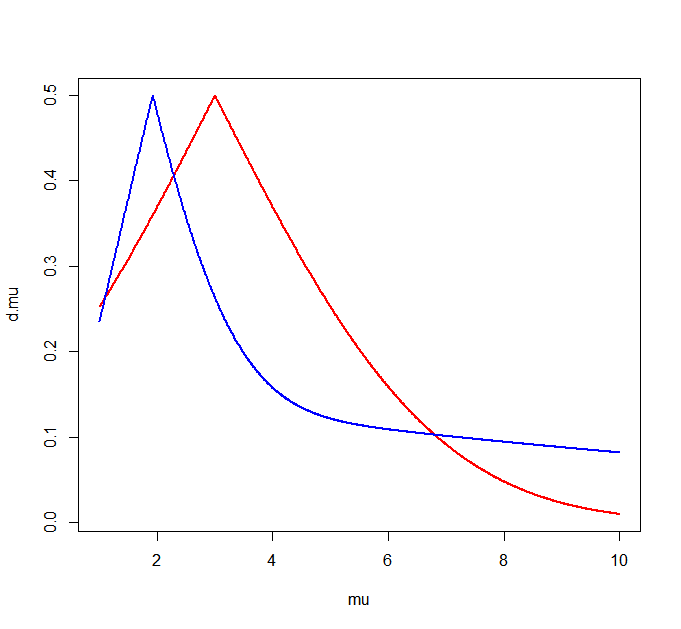
\includegraphics[height=5cm]{depth1.png}
   \label{fig:fig1}
\end{center}
\end{figure}

\paragraph{$N(\mu,f(\mu))$ case} Assume now $f(\mu)>0\quad\forall\quad \mu\in\mathbb{R}$ differentiable. Then we have
\begin{eqnarray*}
-l(\mu,y) &=& \frac{(y-\mu)^2}{2f(\mu)} + \frac{\log f(\mu)}{2} + K\\
\Rightarrow -\frac{dl(y,\mu)}{d\mu} &=& -\frac{(y-\mu)^2f'(\mu)}{2f^2(\mu)} -\frac{y-\mu}{f(\mu)} + \frac{f'(\mu)}{2f(\mu)}\\
&=& \frac{-y^2+2y\mu-\mu^2-2yf(\mu)+2\mu f(\mu)+f(\mu)f'(\mu)}{2f^2(\mu)}\\
&=& \frac{-y^2f'(\mu) + 2y(\mu f'(\mu)-f(\mu)) - [\mu^2f'(\mu)-2\mu f(\mu)-f(\mu)f'(\mu)]}{2f^2(\mu)}\\
&=& -\frac{(y-r_1)(y-r_2)}{2f^2(\mu)}
\end{eqnarray*}
with $r_1, r_2$ being the two roots of the quadratic form in numerator:
$$ r_1,r_2 = \frac{\mu f'(\mu)-f(\mu)\pm\sqrt{(\mu f'(\mu)-f(\mu))^2-\mu^2f'(\mu)+2\mu f(\mu)+f(\mu)f'(\mu)}}{f'(\mu)} = ....$$

Proceeding similarly as the first case, we can conclude that the depth at $\mu$ will be
$$ d(\mu) = \min\left\lbrace P\left[y\in(r_{(1)},r_{(2)})\right], 1-P\left[y\in(r_{(1)},r_{(2)})\right] \right\rbrace $$

\paragraph{General location-scale family} Same assumption $\sigma = k(\mu)$ and density $\exp(g(.))$. Then we have the negative log-likelihood:
\begin{eqnarray*}
-l(\mu,y) &=& -g\left(\frac{y-\mu}{k(\mu)}\right) + \log k(\mu)\\
\quad\Rightarrow\quad -\frac{dl(y,\mu)}{d\mu}  &=& \frac{y-\mu}{k^2(\mu)}+\frac{1}{k(\mu)}\left[g'\left(\frac{y-\mu}{k(\mu)}\right)+ k'(\mu)\right]\\
\end{eqnarray*}

And the student depth comes out to be
\begin{align*}
d(\mu) = \min\left\lbrace P[y-\mu+k(\mu)\tau(\mu;y)+k(\mu)k'(\mu) \geq 0], \right.\nonumber\\
\left. P[y-\mu+k(\mu)\tau(\mu;y)+k(\mu)k'(\mu) \leq 0] \right\rbrace
\end{align*}

with $\tau(\mu;y) = g((y-\mu)/k(\mu))$.

\section{Empirical Likelihood depth}
Tangent depth as per Mizera:
$$ d(\theta) = \frac{1}{n}\min_{u\neq 0} \{\# i: u^Tl_i'(\theta)\geq 0\} $$

with $l_i(\theta)$ being the log-likelihood corresponding to the $i^{th}$ observation. In place of a parametric likelihood, we consider the empirical log-likelihood in the lines of Qin and Lawless, so that information about $P_\theta$ is obtained by $r$ unbiased estimating eqns $g(X,\theta) = (g_1(X,\theta),...,g_r(X,\theta))'$, with $Eg(X,\theta)=0$. Thus we now have (See Qin, Lawless) for $i=1,...,n$

$$ l_i(\theta) = \log\left[1+t^Tg(x_i,\theta)\right] $$
$t = t(\theta)\in\mathbb R^d$ being the solution of the equation
\begin{equation}
\sum_{i=1}^n \frac{g(x_i,\theta)}{1+t^Tg(x_i,\theta)} = 0_{d\times 1}
\end{equation}

Hence we define the \textbf{Empirical likelihood depth} as
$$d_e(\theta) = \frac{1}{n}\min_{u\neq 0} \left\{\#i:u^T\left(\frac{G(x_i,\theta)t}{1+t^Tg(x_i,\theta)}\right)\geq 0\right\}$$

with $t$ satisfying (1) and $G(x,\theta)\in\mathbb{R}^{p\times r}$ being the derivative matrix of $g^T(x,\theta)$ wrt $\theta$.

\paragraph{$p=1$ case} For a single parameter $\theta$, we shall have
$$ d_e(\mu) = \frac{1}{n} \min\left\{ \left(\#i:\frac{G(x_i,\theta)t}{1+t^Tg(x_i,\theta)}\geq 0\right),
\left(\#i:\frac{G(x_i,\theta)t}{1+t^Tg(x_i,\theta)}\leq 0\right) \right\} $$

\paragraph{Maximum likelihood depth} Define the \textbf{Maximum empirical depth estimator} (MEDE) as the value of $\theta$ which maximizes the empirical likelihood depth evaluated there:
$$ \hat{d_e}(\theta) = \argmax_\theta d_e(\theta) = \argmax_\theta \inf_{u\neq 0} P_n\left[u^T\left(\frac{G(x,\theta)t}{1+t^Tg(x,\theta)}\right)\geq 0\right]$$
subject to the constraint (1).

\paragraph{Single parameter: univariate location problem} $X_1,...,X_n\sim F(x-\mu)$ iid; $\mu\in\mathbb{R}, g(X,\theta) = X-\mu$. Then $l_i(\mu) = \log[1+t(x_i-\mu)]$, subject to (1). Hence
$$ d_e(\mu) = \frac{1}{n} \min\left\{ \left(\#i:\frac{t}{1+t(x_i-\mu)}\geq 0\right),
\left(\#i:\frac{t}{1+t(x_i-\mu)}\leq 0\right) \right\} $$

For a given $\mu$ we first solve for $t$ from (1), then obtain the 'depth'. Solving for $t$ is equivalent to minimizing $-\sum_i\log[1+tg(x_,\mu)]$. That can be done by Newton's method close to the actual mean $\mu_0$, but if $\mu$ is far away it's minimized at $\infty$.

\paragraph{Single parameter: multiple estimating equations}
Normal example: $N(\mu,1)$ population. We only know first moment $\mu$, third moment $\mu^3+3\mu$. $g(X,\theta) = (X-\mu,X^3-\mu^3-3\mu)^T$.

$$ d_e(\mu) = \frac{1}{n} \min\left\{ \left(\#i:\frac{t_1+(3\mu^2+3\mu)t_2}{1+t^Tg(x_i,\mu)}\geq 0\right), \left(\#i:\frac{t_1+(3\mu^2+3\mu)t_2}{1+t^Tg(x_i,\mu)}\leq 0\right) \right\} $$


\end{document}